%
% nichtdiff.tex
%
% (c) 2024 Prof Dr Andreas Müller
%
\begin{figure}
\centering
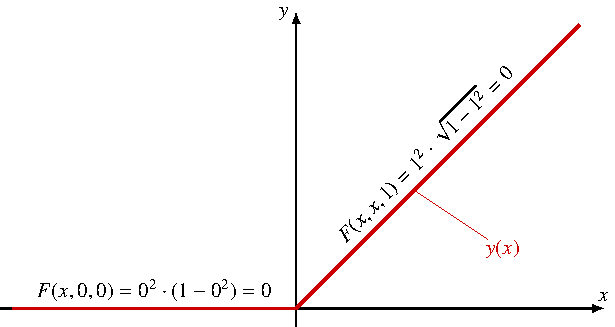
\includegraphics{chapters/030-nichtdiff/images/nichtdiff.pdf}
\caption{Nicht differenzierbare Lösung des Variationsproblems zum
Funktional \eqref{buch:nichtdiff:eckenbedingung:eqn:l} mit
den Randbedingungen $y(-1)=0$ und $y(1)=1$.
\label{buch:nichtdiff:fig:nichtdiff}}
\end{figure}
